\documentclass[12pt]{article}
\usepackage{setspace}
\usepackage{graphicx}
\setstretch {1.25} 
\usepackage{geometry}
\geometry{papersize={21cm,29.7cm}}
\geometry{left=2.5cm,right=2.5cm,top=3cm,bottom=3cm}
\usepackage{fancyhdr}
\usepackage{listings}
\usepackage{color}
\definecolor{black}{rgb}{0,0,0}
\definecolor{olivegreen}{RGB}{112,161,71}
\definecolor{lakeblue}{RGB}{0,127,255}
\definecolor{orange}{RGB}{255,139,0}
\definecolor{purple}{RGB}{102,0,255}
\pagestyle{fancy}
\lhead{\author}
\chead{\date}
\lfoot{}
\cfoot{\thepage}
\rfoot{}
\renewcommand{\headrulewidth}{0.4pt}
\renewcommand{\headwidth}{\textwidth}
\renewcommand{\footrulewidth}{0pt}
\usepackage{xeCJK}
\setCJKmainfont{SimSun}
\XeTeXlinebreaklocale “zh”
\XeTeXlinebreakskip = 0pt plus 1pt
\title{OpenGL作业报告\  C类第1题}
\author{夏斐 2012011417}

\date{\today}
\begin{document}
\maketitle
\linespread {1}
\section{实验环境}
本作业在Mac OS X10.8.2系统下用Xcode完成,程序框架是命令行,用到了系统原生支持的OpenGL和GLUT框架,如图所示:
\begin{center}
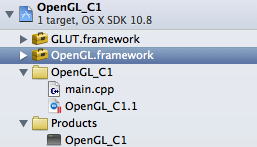
\includegraphics[width = 2.5in]{environment.png} 
\end{center}
\par
\section{实验原理}
这个实验涉及到的原理有openGL的基本图形绘制,OpenGL显示函数,OpenGL空闲函数,双缓冲的概念,变换。
有一个角度量不断更新,然后我们根据角度和平移方向不断在缓冲区中画出这个图案,再交换缓冲区。
\section{实验步骤}
主函数如下:
\begin{lstlisting}[
language=C++, 
breakatwhitespace=false,
label=lst:helloworld, 
caption=Main, 
showspaces=false,
showlines = false,
showstringspaces  = false,
%basicstyle=\ttfamily,
identifierstyle = \color{purple},
stringstyle = \ttfamily,
keywordstyle=\color{lakeblue}\bfseries,
numberstyle = \color{purple}\bfseries,
commentstyle=\color{olivegreen}]

int main(int argc, char ** argv)
{
    glutInit(&argc, argv);   
    glutInitDisplayMode(GLUT_DOUBLE|GLUT_RGBA|GLUT_DEPTH);
    glutInitWindowSize(400 , 400);
    glutInitWindowPosition(100, 100);
    glutCreateWindow("xf");
    glutSetCursor(GLUT_CURSOR_CROSSHAIR);
    glutDisplayFunc(&myDisplay);
    glutIdleFunc(&myDisplay);
    glutMainLoop();
    return 0;
}
\end{lstlisting}
\par
显示函数如下
\begin{lstlisting}[
language=C++, 
breakatwhitespace=false,
label=lst:helloworld, 
caption=Display, 
showspaces=false,
showlines = false,
showstringspaces  = false,
%basicstyle=\ttfamily,
identifierstyle = \color{purple},
stringstyle = \ttfamily,
keywordstyle=\color{lakeblue}\bfseries,
numberstyle = \color{purple}\bfseries,
commentstyle=\color{olivegreen}]
void myDisplay()
{
    glClear(GL_COLOR_BUFFER_BIT|GL_DEPTH_BUFFER_BIT);
    glLoadIdentity();
    glRotatef(angle, 0.0, 0.0, 1.0);
     glTranslatef(-0.5, -0.5, 0);
     glBegin(GL_TRIANGLES);
     glColor3f(1.0, 0, 0);
     glVertex3f(0.0,0.0,0.0);
     glColor3f(0.0, 1, 0);
     glVertex3f(0.7,0.0,0.0);
    glColor3f(0.0, 0.0, 1.0);
    glVertex3f(0.227,0.446,0.0);
     glEnd();
    glutSwapBuffers();
    angle-=0.2;
    
}
\end{lstlisting}

其中采用的参数为我们计算出的三角形坐标的取值,我们先载入恒等矩阵,再做旋转和平移,最终可以保证三角形在自己的内禀坐标系中围绕$(5,5,3)$旋转,着色模式我们选择了SMOOTH。
\par
四边形的显示函数如下:
\begin{lstlisting}[
language=C++, 
breakatwhitespace=false,
label=lst:helloworld, 
caption=Display, 
showspaces=false,
showlines = false,
showstringspaces  = false,
%basicstyle=\ttfamily,
identifierstyle = \color{purple},
stringstyle = \ttfamily,
keywordstyle=\color{lakeblue}\bfseries,
numberstyle = \color{purple}\bfseries,
commentstyle=\color{olivegreen}]
void myDisplay()
{
    if (paint) glShadeModel(GL_SMOOTH);
        else
    glShadeModel(GL_FLAT);
    glClear(GL_COLOR_BUFFER_BIT|GL_DEPTH_BUFFER_BIT);
    glLoadIdentity();
    glRotatef(angle, 0.0, 0.0, 1.0);
    glTranslatef(-0.5, -0.5, 0);

    glBegin(GL_QUADS);
    glColor3f(1.0, 0, 0);
    glVertex3f(0.0,0.0,0.0);
    glColor3f(0.0, 1, 0);
    glVertex3f(0.7,0.0,0.0);
    glColor3f(0.0, 0.0, 1.0);
    glVertex3f(0.227,0.446,0.0);
    glColor3f(1.0, 1.0, 0.0);
    glVertex3f(0,0.446,1);
    
    glEnd();
    glutSwapBuffers();
    angle+=0.2;
}
\end{lstlisting}
我们用一个键盘事件来切换两种着色模式,按下键盘即可切换着色模式。
\begin{lstlisting}[
language=C++, 
breakatwhitespace=false,
label=lst:helloworld, 
caption=Keyevent, 
showspaces=false,
showlines = false,
showstringspaces  = false,
%basicstyle=\ttfamily,
identifierstyle = \color{purple},
stringstyle = \ttfamily,
keywordstyle=\color{lakeblue}\bfseries,
numberstyle = \color{purple}\bfseries,
commentstyle=\color{olivegreen}]
void processNormalKeys(unsigned char key, int x, int y) {
    
    if (key == ' ')
        paint  = !paint;
}\end{lstlisting}
其中实现的具体细节和三角形大致相同,只是着色模式上不同。也是先载入恒等矩阵,再进行平移和旋转,最后绘图。
\section{效果展示}
三角形效果图:
\begin{center}
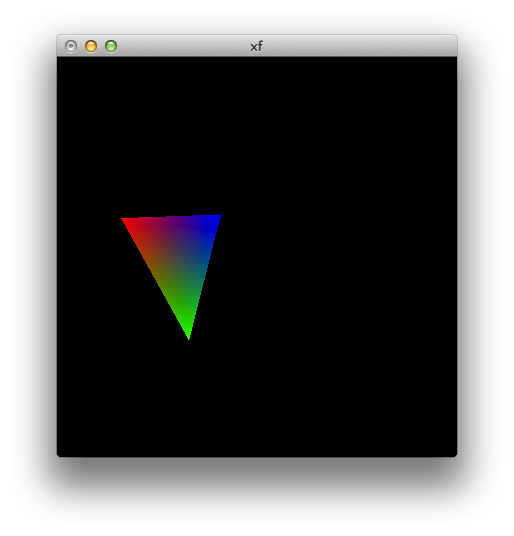
\includegraphics[width = 2.5in]{1.png} 
\end{center}
四边形效果图:
\begin{center}
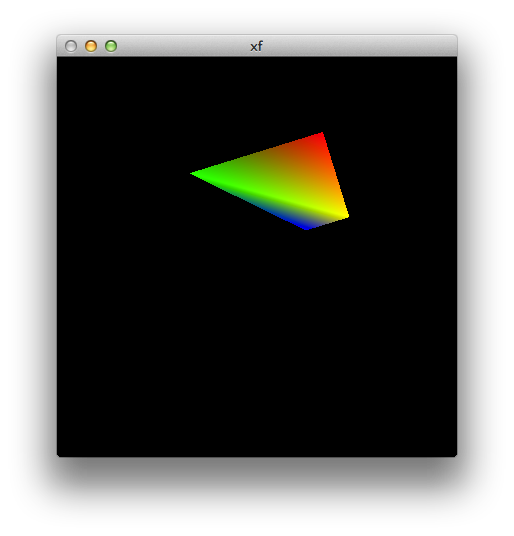
\includegraphics[width = 2.5in]{2.png} 
\end{center}
四边形着色模式FLAT效果图:
\begin{center}
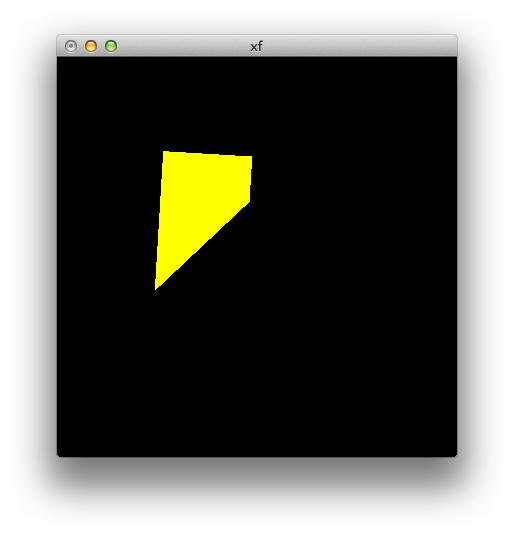
\includegraphics[width = 2.5in]{3.png} 
\end{center}
\section{参考文献}
[1]来自百度文库 OpenGL入门教程(精)
\section{个人信息}
 \noindent
夏斐\\
清华大学 自动化系 2012级\\
手机:(+86)15652799536\\
邮箱:xf1280@gmail.com\\
\end{document}